\documentclass[a4paper,11pt]{article}
\renewcommand*\rmdefault{iwona}
\usepackage[utf8]{inputenc}
\usepackage[square,numbers]{natbib}
\usepackage[T1]{fontenc}
\usepackage{lmodern}
\usepackage{amsmath}
\usepackage{amssymb}
\usepackage{amsthm}
\usepackage{dsfont}
\usepackage{cancel}
\usepackage{graphicx}
\usepackage{geometry}
\usepackage[all]{xy}
\usepackage{graphicx}
\usepackage{microtype}
\usepackage[colorlinks=false, pdfborder={0 0 0}]{hyperref}
\setlength{\parindent}{0pt}

\begin{document}

{
\fontfamily{ppl}\selectfont

~\\

\part*{Compte-rendu Trouvères@Nuit 2016}
Les points importants sont marqués avec une petite étoile [*].

\section{Remarques sur la préparation}
1[*]. Le mieux c'est de désigner quelqu'un motivé dès le début (i.e. dès le premier contact pendant les vacances d'été) comme ``respo Trouvères@Nuit''. Le format d'un concert classique à la Nuit nous semble peu adapté au gala, mais le projet avec les clubs de danse est super.\\
2. La gestion de piano cette année (demande d'autorisation, déplacements, accords) est laissée au COF (@CarolineKM). Tout se passe très bien, il faut juste faire un point sur le piano au buffet (s'il y a besoin et si oui quel piano).\\
3. Les partitions ne sont pas faciles à trouver, et à dire vrai, il n'est pas facile de former un ensemble exprès pour la Nuit en moins de 2 mois (sachant que les premières listes pour les salles de répétitions étaient faites début octobre). Les programmes des années suivantes resteront essentiellement des oeuvres pour piano : @FKaddour était motivée pour monter des pièces de 8 mains, et on peut faire des pubs dans la Plakette $\alpha$.\\
4. Il n'est pas clair au début si l'on peut avoir des remboursements pour les partitions et la procédure est longue. À voir avec le COF si la situation peut s'améliorer.\\
5[**]. Il est crucial qu'on soit au courant de ce qui se passe pour la préparation des salles : @CHuet n'était pas content car on n'était pas aux tests lumières des différentes salles et il a dû changer quelques détails la veille alors qu'on était sans doute stressé. Je n'étais pas du tout au courant de ces tests, mais j'ai reçu des photos de la part de @LudovicM : sauf que tout le monde n'avait pas la même idée sur les placements du quintette, d'où le problème de l'éclairage qui nous a un peu énervé. @LouisD disait que c'est un problème de communication : mettre le respo Trouvères@Nuit sur un mailing liste d'orgas/sous-orgas peut être une solution efficace, mais si l'on ne mérite pas ce statut, tenez-nous au courant de tous les détails qui peuvent éventuellement nous concerner.\\
6. De même pour les lampes de pupitre mais c'était bien passé (in extremis certes).\\
7. On a profité de quelques soirées danses (soirée Tango, soirée multidanses) pour essayer le piano en salle des Actes en guise de répétition : c'était pas mal passé et c'était plutôt apprécié. Le club Tango est motivé pour que ce soit fait plus souvent dans l'année : c'est difficile mais peut-être on peut faire quelques choses aux 48h des arts, ou bien travailler sérieusement sur une petite choréographie.\\
8. Au final, il n'y a pas assez de musiciens motivés. Il faut faire passer l'idée que le gala de l'ENS n'est pas pour les pros : les conscrits sont plutôt persuadés que les gens dansent super bien et ils ont peur de jouer : mais d'après les discussions (je ne connais pas grand chose en danse) ce n'est pas le cas et l'ambiance est plutôt bon enfant.

\section{Remarques sur le déroulement}
1. Il serait peut-être bien de nous laisser répéter une fois dans les salles après l'installation. Mais il est vrai qu'on n'a pas trop de temps.\\
2. Pour le buffet, je n'y étais pas mais d'après @JessicaJ, les gens demandent sans cesse qu'ils augmentent le volume de l'ampli.\\
3. Pour le concert en salle des Actes, au piano solo il faut vraiment jouer fort car au fond on n'entend pas grand chose.\\
4. Pour le concert en Beckett, la salle est beaucoup trop petite mais l'acoustique me semble pas mal. Emplacement du piano à revoir (histoire de sortie de secours).\\
5. Entrée sans fouiller les instruments = cool. Instruments stockés dans un espace dédié au vestiaire et accès prioritaire = cool. Certains musiciens préfèrent ne pas stocker les instruments au vestiaire mais c'est leur choix.\\
6[*]. J'étais trop content de voir les créneaux Trouvères sur le programme imprimé ! Même si finalement pour des problèmes logistiques (lampes de pupitre, difficulté de déplacements des instruments, temps d'installation, discours et présentation du programme) on a 30 mins de retard sur le Tango. Il faudrait donc faire des concerts de moins de 30 mins pour ne pas risquer de trop déborder.\\
7. Les danseurs, nombreux, dansent trop près des instrumentistes et certains musiciens ont peur qu'on abîme leurs instruments précieux. Je ne vois pas de solution (mettre une barrière lol) à part demander sans cesse aux gens de faire attention. De même, les stands soft devraient être placés loin de là où l'on joue (ce qui est bien respecté cette année).\\
8. Cette année on joue une pièce de @KBeffa, on a enregisté mais ça lui fera sans doute plaisir si l'on arrive à filmer. Bref je ne pense pas l'année prochaine qu'on jouera d'oeuvres de compositeurs qu'on connait de toute façon\dots

}
\begin{center}
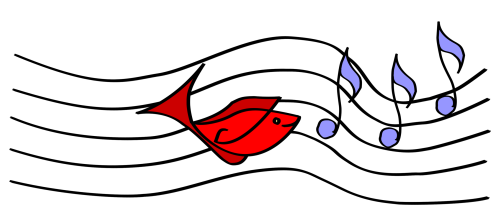
\includegraphics[scale=3]{logo.png}
\end{center}
\begin{center}
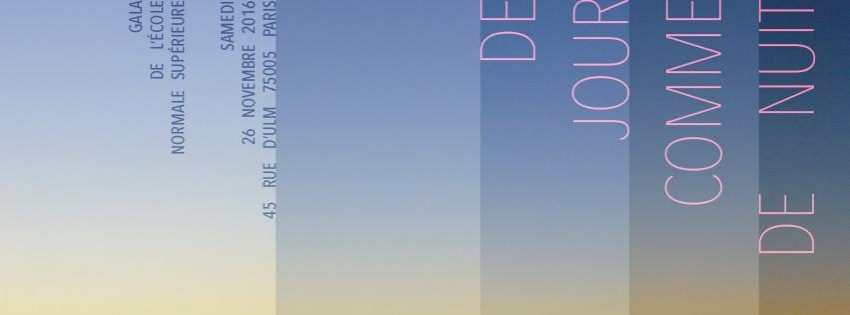
\includegraphics[scale=0.3]{logoNuit.jpg}
\end{center}

\end{document}